\documentclass[tikz=true]{standalone}
\usepackage{amsmath}
\usepackage{tikz}



\usetikzlibrary {arrows, calc,positioning,shapes.misc, graphs, quotes}
\tikzset{terminal/.style={
                          % The shape:
                          rectangle,minimum size=6mm,rounded corners=3mm,
                          % The rest
                          very thick,draw=black!40,
                          top color=white,bottom color=gray!30,
                          }}

\begin{document}
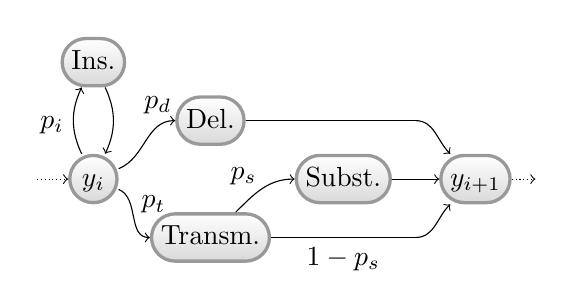
\begin{tikzpicture}[
                    node distance=5mm,
                    text height=1.5ex,text depth=.25ex]
  \matrix[row sep=1mm,column sep=3mm] {
    % First row:
    &\node (ins) [terminal] {Ins.}; & & &  && \\
    % Second row:
     && \node (del) [terminal] {Del.}; & & \node (delToyi1) [coordinate] {}; && \\
    % Third row:
     \node(toyi) [coordinate] {}; &\node (yi) [terminal] {$y_i$}; & & \node (subs) [terminal] {Subst.}; &  &  \node (yi1) [terminal] {$y_{i + 1}$};& \node(fromyi1)[coordinate] {};\\
    % Fourth row:
     && \node (trans) [terminal] {Transm.};& & \node(transToyi1) [coordinate] {}; && \\    
  };

    \graph [edge quotes=auto] {
        (toyi) ->[densely dotted] (yi);
        (yi) ->["$p_i$", out=115, in=-115] (ins) ->[out=-65, in=65] (yi);
        (yi) ->["$p_d$", out=22.5, in=180, edge quotes={above=2pt, near end}] (del) -- (delToyi1) ->[out=0, in=135] (yi1);
        (yi) ->["$p_t$", out=-22.5, in=180, edge quotes={right=1pt, near start}] (trans);
        (trans) -- ["$1 - p_s$", edge quotes=below] (transToyi1) ->[out=0, in=-135] (yi1);
        (trans) ->["$p_s$", out=45, in=180, edge quotes={above left=-2pt}] (subs) -> (yi1);
        (yi1) ->[densely dotted] (fromyi1);
    };
\end{tikzpicture}
    

\end{document}
